% !TeX root = ../../main.tex
\section{Choice of separator}
A crystallisation system consisting of a melt crystalliser (S104) and a subsequent hydraulic wash column (S106) has been chosen as the appropriate separation technique. A PFD for this system is available in Figure \ref{fig:separator PFD}

%Both units have been modelled to determine appropriate dimensions and evaluate the performance of the units. A sensitivity analysis has been conducted on variables with uncertainty to demonstrate its effect on the designs and the output. Finally, mechanical designs with supplementary CAD drawings of both units are included.

\begin{figure}[h]
    \centering
    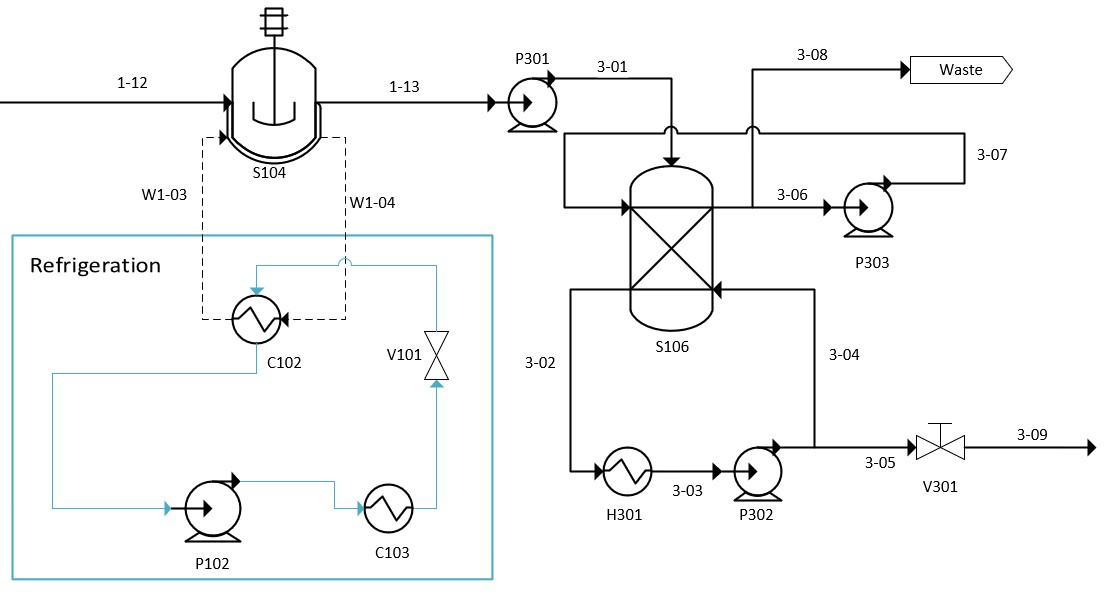
\includegraphics[scale=0.6]{chapters/3-separation/figures/Crystallizer PFD.jpg}
    \caption{PFD of the separation system in consideration; the system consists of a melt crystalliser (S104) and a subsequent hydraulic wash column (S106).}
    \label{fig:separator PFD}
\end{figure}

Due to the small difference in boiling points between nitrotoluene isomers, distillation is infeasible and energy intensive. Similar solubility in both aqueous and organic solvents between the isomers made the use of absorption or adsorption processes infeasible as well. However, crystallisation has been deemed feasible due to the sizeable gaps in melting points between the isomers.

*Table of boiling points, melting points and solubility in water or two organics


Crystallisation can produce high purity products with very low energy input compared to processes like distillation. The heat of transition in crystallisation is typically two to five times lower than in distillation \cite{noauthor_melt_nodate}, which is ideal. In the industry, there are two main processes: solution crystallisation and melt crystallisation. For organics like the nitrotoluene isomers considered in this design, this could mean dissolving the isomers in a solvent. When the resultant solution is cooled down, the isomers crystallise out from the solution at different temperatures. The main drawback, however, for such process is that the solvent required could be environmentally-unfriendly; recovering the solvent or disposing of it is potentially costly. Melt crystallisation, on the other hand, directly utilises the difference in melting points of the components. No additional substance needs to be added for this operation. When the liquid mixture of the components is cooled down, for a eutectic-forming system, one of the components will crystallise as pure solid from the liquid mixture. In general, compared to solution crystallisation, crystal growth rates in melt crystallisers are faster \cite{myerson_handbook_2019}. These advantages make melt crystallisation attractive; hence it has been chosen as the separation technique. 

%Melt crystallisers are usually used to separate organic chemicals with favourable melting points, such as in this case. Typically, solution crystallisation consists of the cooling of the mixuture, decrease the components solubility in the solvent. The same effect can also be achieved with antisolvent crystallisation. However In the case of melt crystallisers only solid and liquid phases are involved allowing for smaller volumes which means less capital costs. Compared to solution crystallisers, the growth rate in melt crystalliser is also relatively fast \cite{myerson_handbook_2019}. Therefore, melt crystallisers were found to be more advantageous for separating p-NT from other organic chemicals. 

There are two main types of melt crystallisers in the industry: solid-layer crystalliser and suspension crystalliser. In solid-layer crystallisers, layer of crystal grows perpendicular to a cooled wall into the bulk of the melt also known as the mother liquor. It is usually a multistage purification process. In contrast, in suspension melt crystallisers the crystallisation initiates on cooled surfaces, and the crystals are scraped off. Crystal growth thus occurs on the crystals suspended in the melt \cite{myerson_handbook_2019}. Table \ref{tab:crystallisertype} lists out the advantages and disadvantage of the two main crystalliser types discussed. 

\begin{table}
\caption{Comparison of crystallisers \cite{myerson_handbook_2019} }
\label{tab:crystallisertype}
\begin{tabularx}{\linewidth}{@{}lXX@{}}
\toprule
Type & Advantages                 & Disadvantages                               \\ \midrule
Solid layer & \begin{itemize}[label=+,leftmargin=1em]
  \item Avoids issue with encrustation
  \item Controllable crystal growth rate 
  \item No slurry handling, easy to operate
\end{itemize} & \begin{itemize}[label=-,leftmargin=1em]
  \item The surface area is a limiting factor, so bigger plant sizes is required; high investment costs
  \item Multistage process: increase in energy consumption and plant size 
  \item Usually a batch or semi-batch process
\end{itemize} \\\midrule 
Suspension &  \begin{itemize}[label=+,leftmargin=1em]
  \item Moderate crystal growth and large surface areas 
  \item High purity product in one step, less energy consumption
  \item Relatively compact process
  \item Continuous process possible
\end{itemize} & \begin{itemize}[label=-,leftmargin=1em]
  \item Slurry handling; stirrers are required to avoid sedimentation
  \item Issues with encrustation 
  \item Solid-liquid separation required, which adds an additional operation cost
\end{itemize}
\\\bottomrule
\end{tabularx}
\end{table}

Even though solid-layer crystallisation has its obvious advantages, the fact that it is usually a multistage batch process made it unattractive, for this would contradict Nitroma's aim for achieving continuous operation throughout the plant to eliminate dangers from material handling. In suspension crystallisation, the surface area for the same volume of crystals is approximately two to three orders of magnitude higher than in solid-layer crystallisation \cite{noauthor_types_nodate}. Suspension crystallisation can achieve a high purity in one stage, whilst layer crystallisation would require more stages to achieve the same level of purity; hence, it would consume less energy compared to layer crystallisation. Suspension crystalliser is thus more suitable for the separation in consideration. 

Mixed-suspension mixed-product removal (MSMPR) is a common mode of operation for modelling continuous melt crystallisers; it has been employed for the melt crystalliser in this design. In such operation, perfect mixing is achieved, and the crystalliser operates at outlet conditions to produce a continuous stream of slurry of crystals and mother liquor. In many ways, the MSMPR mode of operation is similar to the CSTR operation for a reactor. 

%In order to obtain p-NT at greater than 90 \% purity it has to be separated from m-NT and o-NT. Conventional solid-liquid separators are typically operated in batch or semi-batch.Since Nitroma aims for a continuous plant these separators were not suitable. For instance, a centrifuge would require  solid material handling possibly using a conveyor belt to transport the solid. This has many difficulties and could become a bottle neck in the entire plant. Alternatively, wash columns were considered as they can be operated continuously and achieve ultrapurification. 

For separating the solid from the liquid, 